\documentclass[UTF8,titlepage]{ctexart}
\usepackage{amsmath,amssymb,amsthm,amsfonts,amscd}
\usepackage{fontspec}
\setmainfont{Times New Roman}
\usepackage{graphicx}
\usepackage{titlesec}
\usepackage{makecell}
\usepackage{longtable}
\usepackage{xcolor}
\usepackage{tcolorbox}
\usepackage{soul}
\usepackage{adjustbox}
\usepackage{tcolorbox}
\usepackage{enumerate}
\usepackage{pdfpages}
\usepackage{float}
\usepackage{colortbl}
\usepackage{tabularx}
\usepackage{multirow}
\usepackage{pgfplots}
\usepackage{minted}
\numberwithin{figure}{section}
\usepackage[left=1.25in,right=1.25in,%
top=1in,bottom=1in]{geometry}
\usepackage{color}
\titleformat{\section}
  {\raggedright\LARGE\bfseries}{\thesection}{1em}{}


\begin{document}
\title{计算机通信网课程设计报告}
\author{赵伯远 211440128}
\date{\today}
\maketitle
\tableofcontents
\clearpage
\section{实验环境}
\begin{itemize}
    \item 操作系统:Ubuntu 20.04.2 LTS
    \item Python版本:3.9.18
    \item Scapy版本:2.4.4
    \item dns.resolver版本:1.1.1
    \item requests版本:2.25.1
    \item BeautifulSoup版本:4.9.3
    \item 实验机1IPv4地址:10.206.17.20
    \item 实验机2IPv4地址:10.206.184.101
\end{itemize}
\section{项目1:子网划分}
\subsection{项目描述}
这个项目旨在实现一个子网划分的工具。用户提供一个基础网络地址、子网掩码和所需的子网数量,程序将自动计算并展示出所有子网的详细信息,包括子网地址、广播地址、可用地址范围和子网掩码。

\subsection{项目实现思路}
实现这个功能,首先需要将用户输入的基础网络地址和子网掩码转换为IP网络对象。随后,根据所需的子网数量计算出新的子网掩码。最后,遍历并打印出每个子网的详细信息。

\subsection{项目代码}
以下是实现子网划分的Python代码:

\begin{minted}[frame=lines,framesep=2mm,baselinestretch=1.2,fontsize=\footnotesize,linenos]{python}
import ipaddress

def subnet_division(network_address, subnet_mask, required_subnets):
    # 将输入的网络地址和子网掩码转换为IP网络对象
    network = ipaddress.ip_network(f"{network_address}/{subnet_mask}", strict=False)

    # 计算新子网掩码
    new_prefix_length = network.prefixlen + (required_subnets - 1).bit_length()

    # 生成和打印子网划分方案
    print("子网划分方案:")
    print(f"{'子网地址':<20}{'广播地址':<20}{'可用地址范围':<40}{'子网掩码':<20}")
    for subnet in network.subnets(new_prefix=new_prefix_length):
        network_address_str = str(subnet.network_address)
        broadcast_address_str = str(subnet.broadcast_address)
        range_start_str = str(subnet.network_address + 1)
        range_end_str = str(subnet.broadcast_address - 1)
        subnet_mask_str = str(subnet.with_netmask.split('/')[1])

        print(f"{network_address_str:<20}{broadcast_address_str:<20}"
            f"{range_start_str} - {range_end_str:<40}"
            f"{subnet_mask_str:<20}")

    # 二进制划分方法展示
    print("\n二进制划分方法:")
    bin_network_address = ''.join(f'{octet:08b}' for octet in subnet.network_address.packed)
    bin_subnet_mask = ''.join(f'{octet:08b}' for octet in subnet.netmask.packed)
    print(f"网络地址(二进制): {bin_network_address}")
    print(f"子网掩码(二进制): {bin_subnet_mask}")

def main():
    # 用户输入
    network_address = input("请输入网络地址(例如:192.168.1.0):")
    subnet_mask = input("请输入子网掩码(例如:255.255.255.0):")
    required_subnets = int(input("请输入所需的网络数:"))

    # 执行子网划分
    subnet_division(network_address, subnet_mask, required_subnets)

if __name__ == '__main__':
    main()
\end{minted}

\subsection{实验结果}
实验结果将展示每个子网的详细信息,包括子网地址、广播地址、可用地址范围和子网掩码。此外,还提供了二进制格式的网络地址和子网掩码以供参考。
\begin{figure}[H]
\centering
 \resizebox{0.75\textwidth}{!}{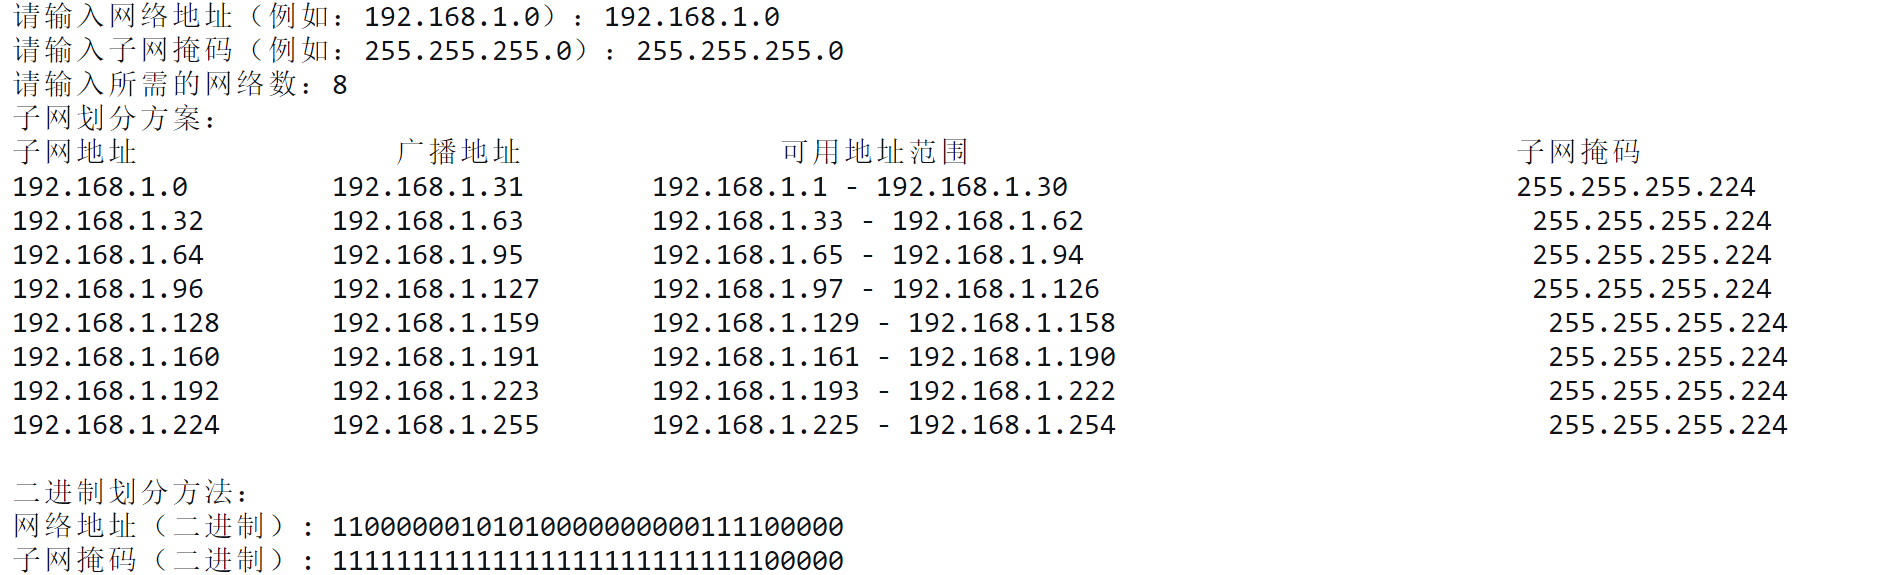
\includegraphics{img/1.png}}
 \caption{子网划分结果}
 \label{}
\end{figure}
\clearpage
\section{项目2:利用 TCP 时间戳选项实现 TCP 协议超时重传计算}

\subsection{项目描述}
本项目的目的是通过利用TCP协议的时间戳选项来计算并实现超时重传(RTO)的动态调整。这对于提高网络通信的可靠性和效率非常重要。

\subsection{项目实现思路}
项目通过创建一个TCP连接并发送数据到服务器,接着测量往返时间(RTT)来实现。利用这些RTT值,我们可以计算平滑的RTT(SRTT),RTT的变化量(RTTVAR),以及基于这些值的重传超时(RTO)。通过不断更新这些值,我们可以更准确地估计何时进行重传。

\subsection{项目代码}
以下是实现TCP超时重传计算的Python代码:

\begin{minted}[frame=lines,framesep=2mm,baselinestretch=1.2,fontsize=\footnotesize,linenos]{python}
import time
import socket

# 参数初始化
alpha = 0.125
beta = 0.25
G = 0.1  # 100毫秒

# 初始RTT、SRTT、RTTVAR和RTO的设定
initial_rtt = 0.5  # 假设的初始RTT值,单位秒
srtt = initial_rtt
rttvar = initial_rtt / 2
rto = srtt + max(G, 4 * rttvar)

# 创建TCP连接
client_socket = socket.socket(socket.AF_INET, socket.SOCK_STREAM)
client_socket.connect(("www.google.com", 80))  # 连接到目标服务器和端口

# 发送和接收数据,计算RTT
try:
    for _ in range(5):  # 发送五次数据进行测试
        send_time = time.time()
        client_socket.sendall(b"GET / HTTP/1.1\r\nHost: www.google.com\r\n\r\n")
        response = client_socket.recv(4096)
        recv_time = time.time()

        # 计算当前RTT
        rtt = recv_time - send_time

        # 更新SRTT和RTTVAR
        rttvar = (1 - beta) * rttvar + beta * abs(srtt - rtt)
        srtt = (1 - alpha) * srtt + alpha * rtt

        # 更新RTO
        rto = srtt + max(G, 4 * rttvar)

        print(f"RTT: {rtt:.3f}, SRTT: {srtt:.3f}, RTTVAR: {rttvar:.3f}, RTO: {rto:.3f}")

finally:
    client_socket.close()
\end{minted}

\subsection{实验结果}
实验结果将展示每次通信的RTT、SRTT、RTTVAR和RTO的值。这些数据帮助理解和验证TCP超时重传计算的效果。
\begin{figure}[H]
\centering
 \resizebox{0.75\textwidth}{!}{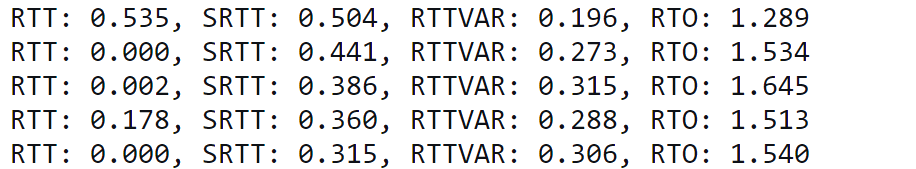
\includegraphics{img/2.png}}
 \caption{TCP超时重传计算结果}
 \label{}
\end{figure}
\clearpage
\section{项目3:Traceroute 程序实现}
\subsection{项目描述}
本项目的目的是实现一个简单的 Traceroute 程序,用于跟踪数据包在网络中传输的路径。这个工具可以帮助诊断网络连接问题,通过展示数据包到达目的地所经过的每个路由器的地址和往返时间。

\subsection{项目实现思路}
Traceroute 程序通过发送 ICMP Echo 请求消息,并逐步增加 IP 包的生存时间(TTL)来实现。每当数据包到达一个路由器,其 TTL 就会减少 1,当 TTL 减少到 0 时,路由器会发送一个 ICMP 超时响应回来。通过这种方式,我们可以追踪数据包的路径。

\subsection{项目代码}
以下是实现 Traceroute 功能的 Python 代码:


\begin{minted}[frame=lines,framesep=2mm,baselinestretch=1.2,fontsize=\footnotesize,linenos]{python}
import os
import socket
import struct
import time
import select

# 您已有的 checksum 函数保持不变
def checksum(source_string):
    """
    计算校验和
    """
    sum = 0
    max_count = (len(source_string)/2)*2
    count = 0
    while count < max_count:
        val = source_string[count + 1]*256 + source_string[count]
        sum = sum + val
        sum = sum & 0xffffffff 
        count = count + 2
     
    if max_count < len(source_string):
        sum = sum + source_string[len(source_string) - 1]
        sum = sum & 0xffffffff 
    
    sum = (sum >> 16) + (sum & 0xffff)
    sum = sum + (sum >> 16)
    answer = ~sum
    answer = answer & 0xffff
    answer = answer >> 8 | (answer << 8 & 0xff00)
    return answer

def create_packet(id):
    """
    创建 ICMP Echo 请求包
    """
    header = struct.pack('bbHHh', 8, 0, 0, id, 1)
    data = 192 * b'Q'
    my_checksum = checksum(header + data)
    header = struct.pack('bbHHh', 8, 0, socket.htons(my_checksum), id, 1)
    return header + data

def traceroute(host, max_hops=30, timeout=10):
    """
    实现 traceroute 功能
    """
    try:
        dest_addr = socket.gethostbyname(host)
    except socket.gaierror:
        print(f"无法解析主机: {host}")
        return

    print(f"Traceroute to {host} [{dest_addr}], {max_hops} hops max")

    icmp = socket.getprotobyname("icmp")
    for ttl in range(1, max_hops + 1):
        try:
            sock = socket.socket(socket.AF_INET, socket.SOCK_RAW, icmp)
            sock.setsockopt(socket.SOL_IP, socket.IP_TTL, struct.pack('I', ttl))
            sock.settimeout(timeout)
        except socket.error as e:
            print(f"无法创建 socket: {e}")
            break

        packet_id = os.getpid() & 0xFFFF
        packet = create_packet(packet_id)

        try:
            sock.sendto(packet, (dest_addr, 1))
            start_time = time.time()
            ready = select.select([sock], [], [], timeout)
            if ready[0] == []:
                print(f"{ttl} 请求超时")
            else:
                received_packet, addr = sock.recvfrom(1024)
                time_received = time.time()
                rtt = (time_received - start_time) * 1000
                print(f"{ttl} 来自 {addr[0]}: 字节={len(received_packet)} 时间={round(rtt, 2)}ms")

                if addr[0] == dest_addr:
                    print("达到目标主机")
                    break
        except socket.error as e:
            print(f"发送或接收数据时发生错误: {e}")
        finally:
            sock.close()

        time.sleep(1)

if __name__ == "__main__":
    traceroute("www.baidu.com")


\end{minted}

\subsection{实验结果}
实验结果将展示从本机到目标主机的每一跳的IP地址和往返时延。这有助于分析和理解数据在网络中的传输路径。
\begin{figure}[H]
\centering
 \resizebox{0.75\textwidth}{!}{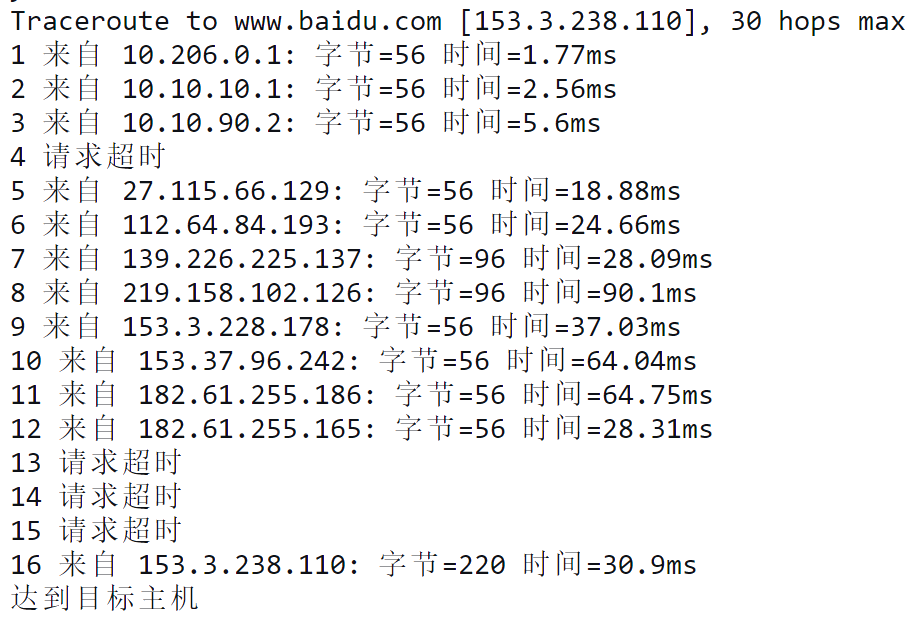
\includegraphics{img/3.png}}
 \caption{Traceroute结果}
 \label{}
\end{figure}

\clearpage

\section{项目:Ping 程序实现}

\subsection{项目描述}
本项目的目标是实现一个简单的 Ping 程序。Ping 是一种网络工具,用于测试数据包是否能通过IP网络发送到特定主机,并且主机能否回复。这个程序将模拟 Ping 的基本功能,它发送 ICMP Echo 请求给目标主机,并等待 Echo 响应来测量往返时间(RTT)。

\subsection{项目实现思路}
项目使用 Python 语言和标准库实现。首先,程序通过 DNS 解析获取目标主机的 IP 地址。然后,创建 ICMP Echo 请求包,并通过原始套接字发送这些包。程序使用 select 来等待响应,并计算接收响应的时间以测量 RTT。该过程重复几次,以提供准确的测量结果。

\subsection{项目代码}
以下是实现 Ping 程序的 Python 代码:

\begin{minted}[frame=lines,framesep=2mm,baselinestretch=1.2,fontsize=\footnotesize,linenos]{python}
import os
import socket
import struct
import time
import select

def checksum(source_string):
    """
    计算校验和
    """
    sum = 0
    max_count = (len(source_string)/2)*2
    count = 0
    while count < max_count:
        val = source_string[count + 1]*256 + source_string[count]
        sum = sum + val
        sum = sum & 0xffffffff 
        count = count + 2
     
    if max_count < len(source_string):
        sum = sum + source_string[len(source_string) - 1]
        sum = sum & 0xffffffff 
    
    sum = (sum >> 16) + (sum & 0xffff)
    sum = sum + (sum >> 16)
    answer = ~sum
    answer = answer & 0xffff
    answer = answer >> 8 | (answer << 8 & 0xff00)
    return answer

def create_packet(id):
    """
    创建 ICMP Echo 请求包
    """
    header = struct.pack('bbHHh', 8, 0, 0, id, 1)
    data = 192 * b'Q'
    my_checksum = checksum(header + data)
    header = struct.pack('bbHHh', 8, 0, socket.htons(my_checksum), id, 1)
    return header + data

def ping(host, timeout=1, count=4):
    """
    发送 ping 请求
    """
    try:
        dest_addr = socket.gethostbyname(host)
    except socket.gaierror:
        print(f"无法解析主机: {host}")
        return

    print(f"Pinging {host} [{dest_addr}] with {count} packets of data:")

    for i in range(count):
        icmp = socket.getprotobyname("icmp")
        try:
            sock = socket.socket(socket.AF_INET, socket.SOCK_RAW, icmp)
        except socket.error as e:
            print(f"无法创建 socket: {e}")
            return

        packet_id = os.getpid() & 0xFFFF
        packet = create_packet(packet_id)

        try:
            sock.sendto(packet, (dest_addr, 1))
            start_time = time.time()
            ready = select.select([sock], [], [], timeout)
            if ready[0] == []:
                print("请求超时")
            else:
                received_packet, addr = sock.recvfrom(1024)
                time_received = time.time()
                rtt = (time_received - start_time) * 1000
                print(f"来自 {addr[0]}: 字节={len(received_packet)} 时间={round(rtt, 2)}ms")
        except socket.error as e:
            print(f"发送或接收数据时发生错误: {e}")
        finally:
            sock.close()
        time.sleep(1)

if __name__ == "__main__":
    ping("www.baidu.com")
\end{minted}

\subsection{实验结果}

实验结果将展示对目标主机发出的每个 Ping 请求的响应时间。这将帮助用户了解网络连接的质量和稳定性。
\begin{figure}[H]
\centering
 \resizebox{0.75\textwidth}{!}{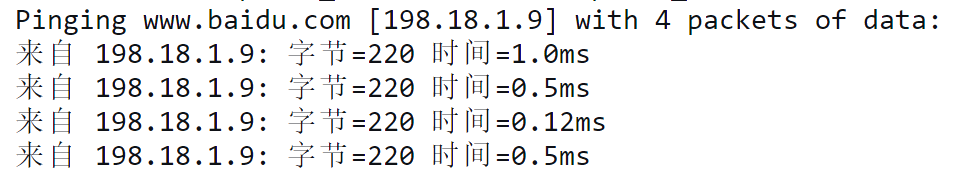
\includegraphics{img/4.png}}
 \caption{Ping结果}
 \label{}
\end{figure}

\clearpage
\section{项目5:TCP 三报文握手建立连接、四报文挥手释放连接程序实现}

\subsection{项目描述}
本项目旨在通过编程模拟 TCP 协议的关键特性:三次握手和四次挥手。三次握手是建立 TCP 连接的过程,而四次挥手是断开已建立的 TCP 连接的过程。该项目通过编写脚本来模拟这两个过程,从而深入理解 TCP 协议的工作原理。

\subsection{项目实现思路}
项目使用 Python 语言和 Scapy 库来实现。首先,发送一个 SYN 报文并等待 SYN-ACK 响应,完成三次握手的前两个步骤。接着,发送 ACK 报文完成握手。然后,发送 FIN 报文并等待服务器的 FIN-ACK 响应,完成四次挥手的前两个步骤。最后,发送最后的 ACK 报文以彻底断开连接。

\subsection{项目代码}
以下是实现 TCP 三报文握手和四报文挥手的 Python 代码:

\begin{minted}[frame=lines,framesep=2mm,baselinestretch=1.2,fontsize=\footnotesize,linenos]{python}
from scapy.all import *
import time

def tcp_handshake(target_ip, target_port):
    # 构造IPv4 SYN报文
    ip = IP(dst=target_ip)
    syn = TCP(sport=RandShort(), dport=target_port, flags="S")
    syn_ack = sr1(ip/syn, timeout=1)

    # 检查是否收到IPv6 SYN-ACK响应
    if syn_ack and syn_ack.haslayer(TCP) and syn_ack.getlayer(TCP).flags & 0x12:
        # 发送IPv6 ACK报文
        ack = TCP(sport=syn.sport, dport=target_port, flags="A", seq=syn_ack.ack, ack=syn_ack.seq + 1)
        send(ip/ack)
        print("TCP三次握手完成")
        return syn_ack.seq + 1, ack.seq
    else:
        print("握手失败")
        return None, None

def tcp_teardown(target_ip, target_port, seq, ack_seq):
    # 发送FIN报文
    ip = IP(dst=target_ip)
    fin = TCP(sport=RandShort(), dport=target_port, flags="FA", seq=seq, ack=ack_seq)
    send(ip/fin)

    # 接收服务器响应并丢弃RST报文
    ans, _ = sr(ip/TCP(sport=fin.dport, dport=fin.sport, flags="A"), timeout=1, verbose=False)
    
    if ans and ans[0][1].haslayer(TCP):
        tcp_layer = ans[0][1].getlayer(TCP)
        if tcp_layer.flags & 0x04:  # 检查是否是 RST
            print("收到RST,但已丢弃")
        else:
            print("未收到RST")

    # 发送最后的ACK报文
    last_ack = TCP(sport=fin.sport, dport=target_port, flags="A", seq=tcp_layer.ack, ack=tcp_layer.seq + 1)
    send(ip/last_ack)
    print("TCP四次挥手完成")

if __name__ == "__main__":
    target_ip = "127.0.0.1"  # 目标服务器IP地址
    target_port = 80  # 目标服务器端口
    seq, ack_seq = tcp_handshake(target_ip, target_port)

    if seq and ack_seq:
        time.sleep(2)  # 等待一段时间再开始挥手
        tcp_teardown(target_ip, target_port, seq, ack_seq)
\end{minted}

\subsection{实验结果}
实验结果将展示 TCP 三次握手和四次挥手的过程,包括发送的报文类型、收到的响应以及相应的状态消息。这些结果有助于验证 TCP 连接建立和释放的实现。
\begin{figure}[H]
\centering
 \resizebox{0.75\textwidth}{!}{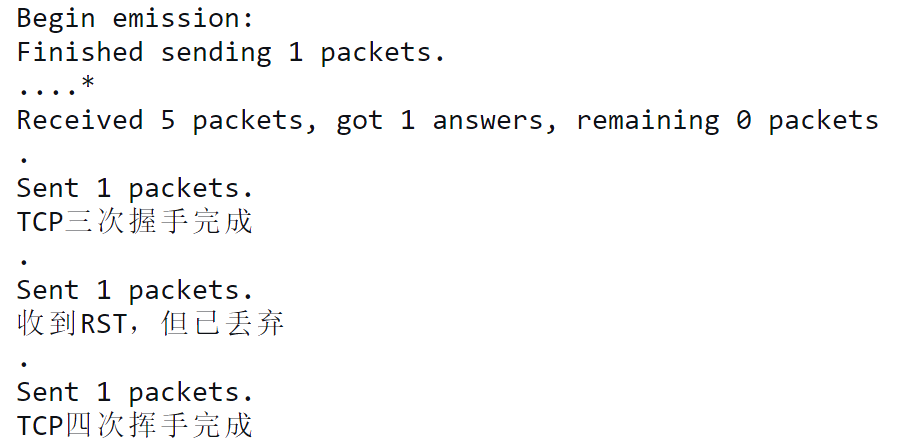
\includegraphics{img/5.png}}
 \caption{TCP三次握手和四次挥手结果}
 \label{}
\end{figure}
\clearpage
\section{项目6:IP 首部检验和计算程序实现}

\subsection{项目描述}
本项目旨在通过编程计算 IP 数据报首部的检验和。IP 首部的检验和是网络通信中保证数据完整性的重要机制,它可以帮助接收端检测在传输过程中是否发生错误。

\subsection{项目实现思路}
项目使用 Python 语言和 Scapy 库来实现。首先,程序将嗅探网络上的 IP 数据报,并提取每个数据报的 IP 首部。然后,使用标准的检验和计算方法来计算这些首部的检验和,并与数据报中的原始检验和进行比较。

\subsection{项目代码}
以下是实现 IP 首部检验和计算的 Python 代码:

\begin{minted}[frame=lines,framesep=2mm,baselinestretch=1.2,fontsize=\footnotesize,linenos]{python}
from scapy.all import sniff, IP
import struct

def checksum(ip_header):
    """
    计算 IP 首部的检验和
    """
    # 将 bytes 类型的 IP 首部转换为可修改的列表
    ip_header = list(ip_header)

    # 将检验和字段(第 10、11 字节)置为 0
    ip_header[10] = 0
    ip_header[11] = 0

    sum = 0
    # 每次取两个字节
    for i in range(0, len(ip_header), 2):
        word = (ip_header[i] << 8) + (ip_header[i + 1])
        sum += word
        sum = (sum & 0xffff) + (sum >> 16)  # 将溢出的部分加到低16位

    return ~sum & 0xffff

def handle_packet(packet):
    """
    处理捕获的 IP 数据报
    """
    if IP in packet:
        ip_header = packet[IP]
        print(f"捕获到 IP 数据报:{ip_header.summary()}")

        # 获取原始的 IP 首部信息
        raw_header = bytes(ip_header)[:20]  # 只取 IP 首部前20字节
        print(f"原始首部信息:{raw_header}")

        # 计算并显示检验和
        calculated_checksum = checksum(raw_header)
        print(f"计算的检验和:{calculated_checksum:04x}")

# 嗅探网络上的 IP 数据报
sniff(filter="ip", prn=handle_packet, count=10)

\end{minted}

\subsection{实验结果}
实验结果将展示捕获到的前10个 IP 数据报的详细信息,包括原始首部信息和计算出的检验和。这有助于验证检验和计算方法的准确性和效率。
\begin{figure}[H]
\centering
 \resizebox{0.75\textwidth}{!}{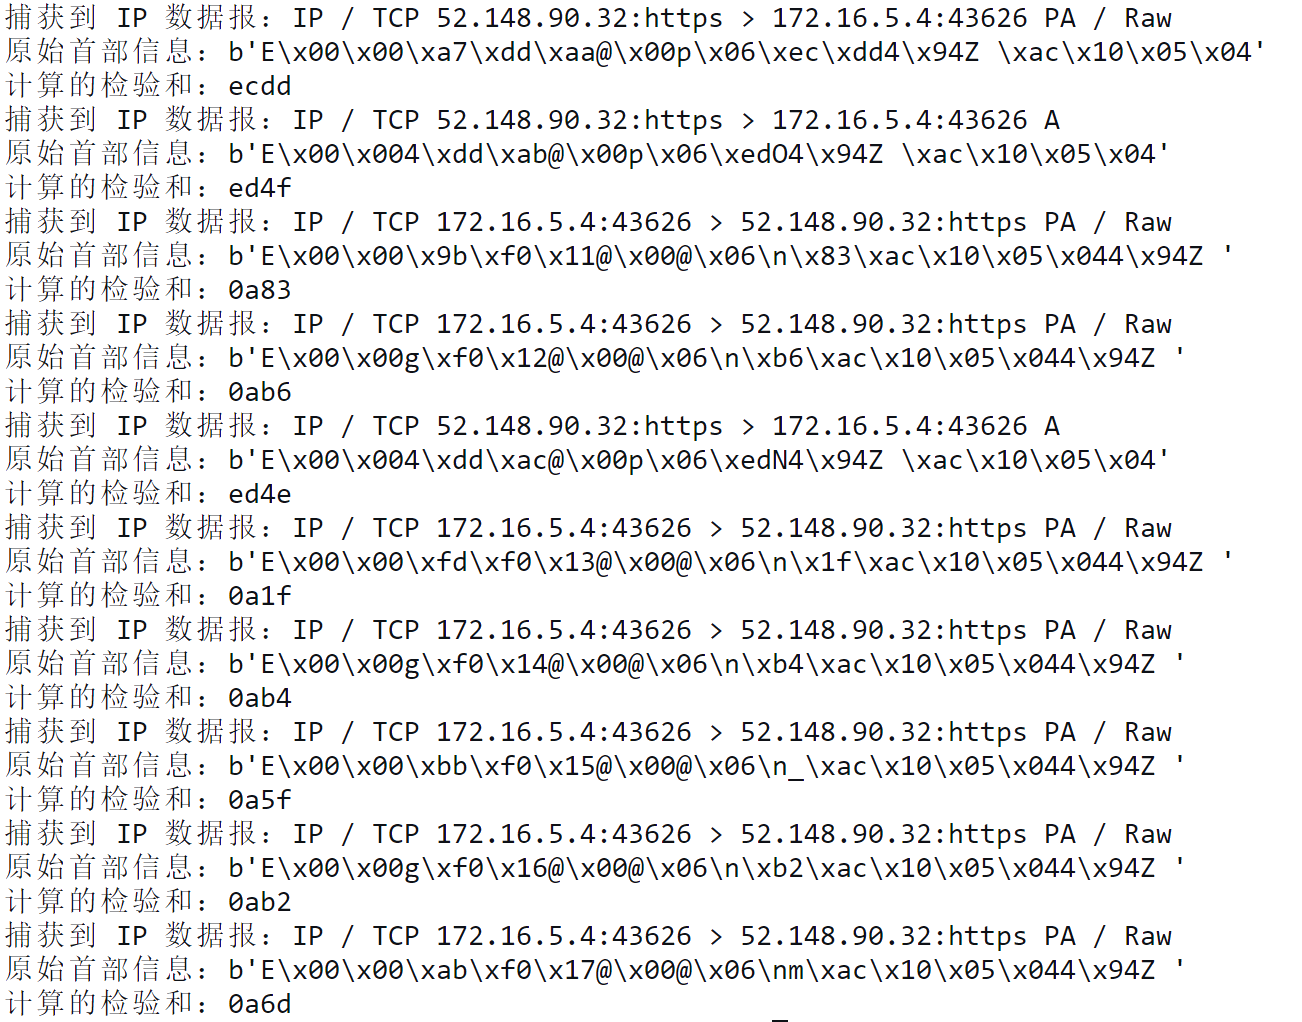
\includegraphics{img/6.png}}
 \caption{IP首部检验和计算结果}
 \label{}
\end{figure}

\clearpage

\section{项目7:主机端口扫描程序设计}

\subsection{项目描述}
本项目的目的是设计并实现一个端口扫描程序,用于检测目标主机上的网络端口状态。这种类型的扫描对于网络安全和管理是非常重要的,可以帮助发现开放的或潜在的脆弱端口。

\subsection{项目实现思路}
项目使用 Python 语言和 Scapy 库来实现端口扫描功能。程序将对目标IP地址的指定端口范围进行扫描,使用 TCP SYN 扫描和 UDP 扫描来检测端口的状态。为了提高扫描效率,程序采用多线程并发处理端口扫描任务。

\subsection{项目代码}
以下是实现端口扫描程序的 Python 代码:

\begin{minted}[frame=lines,framesep=2mm,baselinestretch=1.2,fontsize=\footnotesize,linenos]{python}
from scapy.all import *
import sys
from concurrent.futures import ThreadPoolExecutor

def scan_port(ip, port):
    try:
        # TCP SYN Scan
        syn_pkt = IP(dst=ip) / TCP(dport=port, flags="S")
        response = sr1(syn_pkt, timeout=1, verbose=0)
        if response and response.haslayer(TCP) and response.getlayer(TCP).flags & 0x12:
            return port, 'Open'

        # UDP Scan
        udp_pkt = IP(dst=ip) / UDP(dport=port)
        response = sr1(udp_pkt, timeout=1, verbose=0)
        if not response or (response.haslayer(ICMP) and response.getlayer(ICMP).type != 3):
            return port, 'Open/Filtered'
    except Exception as e:
        return port, 'Error'
    return port, 'Closed'

def scan(ip, ports, max_threads=100):
    with ThreadPoolExecutor(max_workers=max_threads) as executor:
        scan_results = executor.map(lambda p: scan_port(ip, p), ports)
        for port, status in scan_results:
            print(f"Port {port}: {status}")

if __name__ == "__main__":
    target_ip = sys.argv[1] if len(sys.argv) > 1 else "10.206.17.20"
    ports = range(1, 1025)  # Standard range of ports
    scan(target_ip, ports)
\end{minted}

\subsection{实验结果}
实验结果将展示对目标主机端口扫描的详细输出,包括每个端口的状态(如开放、关闭或过滤)。这些结果有助于分析目标主机的网络安全状况。
\begin{figure}[H]
\centering
 \resizebox{0.5\textwidth}{!}{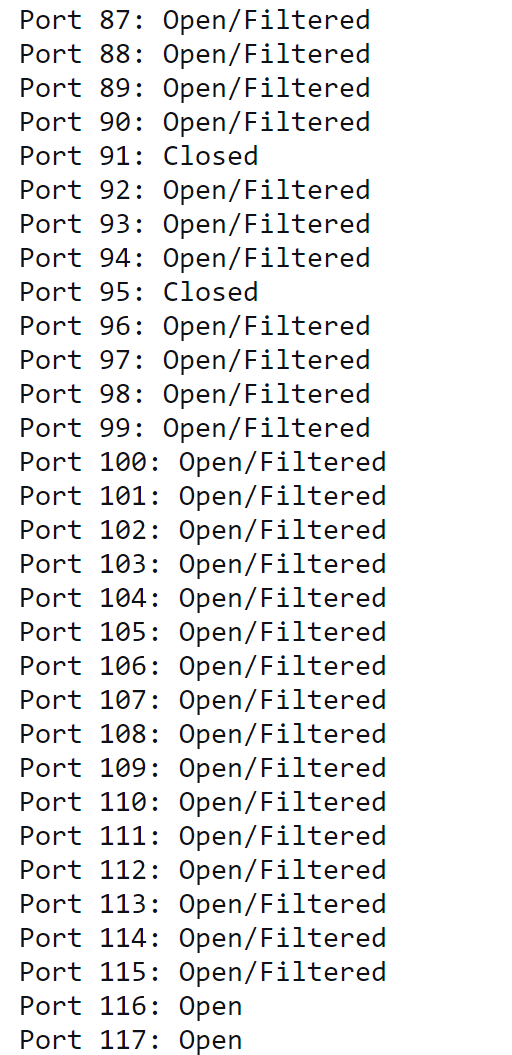
\includegraphics{img/7.png}}
 \caption{端口扫描结果}
 \label{}
\end{figure}
\clearpage

\section{项目8:DNS 解析}

\subsection{项目描述}
本项目的目的是设计并实现一个 DNS 查询工具。DNS(域名系统)是互联网的核心部分,负责将域名转换为 IP 地址。此工具将允许用户对特定域名执行不同类型的 DNS 查询,并从指定的 DNS 服务器获取结果。

\subsection{项目实现思路}
项目使用 Python 语言和第三方库 dns.resolver 来实现。程序将接受域名、查询类型(如 A、NS、SOA、MX、CNAME)和 DNS 服务器地址作为输入,并返回查询结果。这不仅包括记录数据,还包括查询是权威的还是非权威的。

\subsection{项目代码}
以下是实现 DNS 解析的 Python 代码:

\begin{minted}[frame=lines,framesep=2mm,baselinestretch=1.2,fontsize=\footnotesize,linenos]{python}
import dns.resolver

def query_dns(domain, record_type, dns_server):
    resolver = dns.resolver.Resolver()
    resolver.nameservers = [dns_server]

    try:
        answer = resolver.resolve(domain, record_type)
        for rdata in answer:
            print(f"{record_type} Record:", rdata.to_text())
            print("Response is", "authoritative" if answer.response.flags & dns.flags.AA else "non-authoritative")
    except Exception as e:
        print(f"Error querying {domain} for {record_type} record: {e}")

if __name__ == "__main__":
    domain_to_query = "www.github.com"
    dns_server_to_use = "8.8.8.8"  # Google's public DNS server
    record_types = ["A", "NS", "SOA", "MX", "CNAME"]

    for record_type in record_types:
        query_dns(domain_to_query, record_type, dns_server_to_use)
\end{minted}

\subsection{实验结果}
实验结果将展示对指定域名的 DNS 查询输出,包括每种查询类型的记录和其权威性。这将有助于用户理解域名的 DNS 配置和解析过程。
\begin{figure}[H]
\centering
 \resizebox{0.75\textwidth}{!}{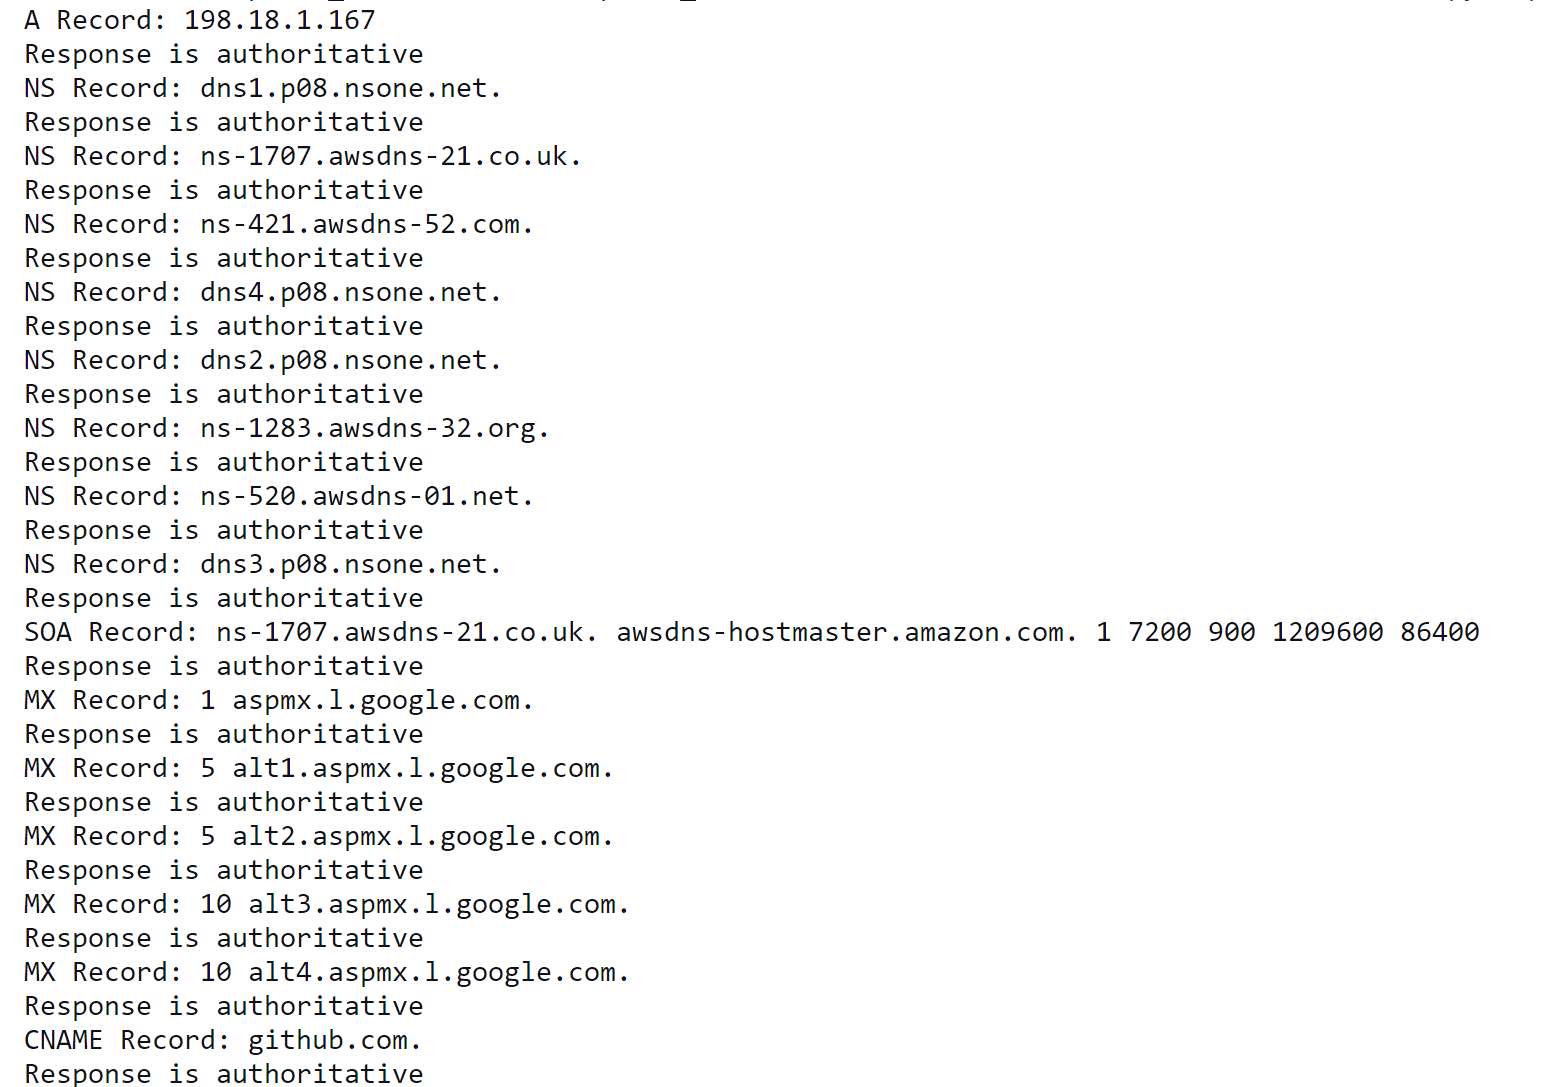
\includegraphics{img/8.1.png}}
 \caption{对www.github.com的DNS解析结果}
 \label{}
\end{figure}

\begin{figure}[H]
\centering
 \resizebox{0.75\textwidth}{!}{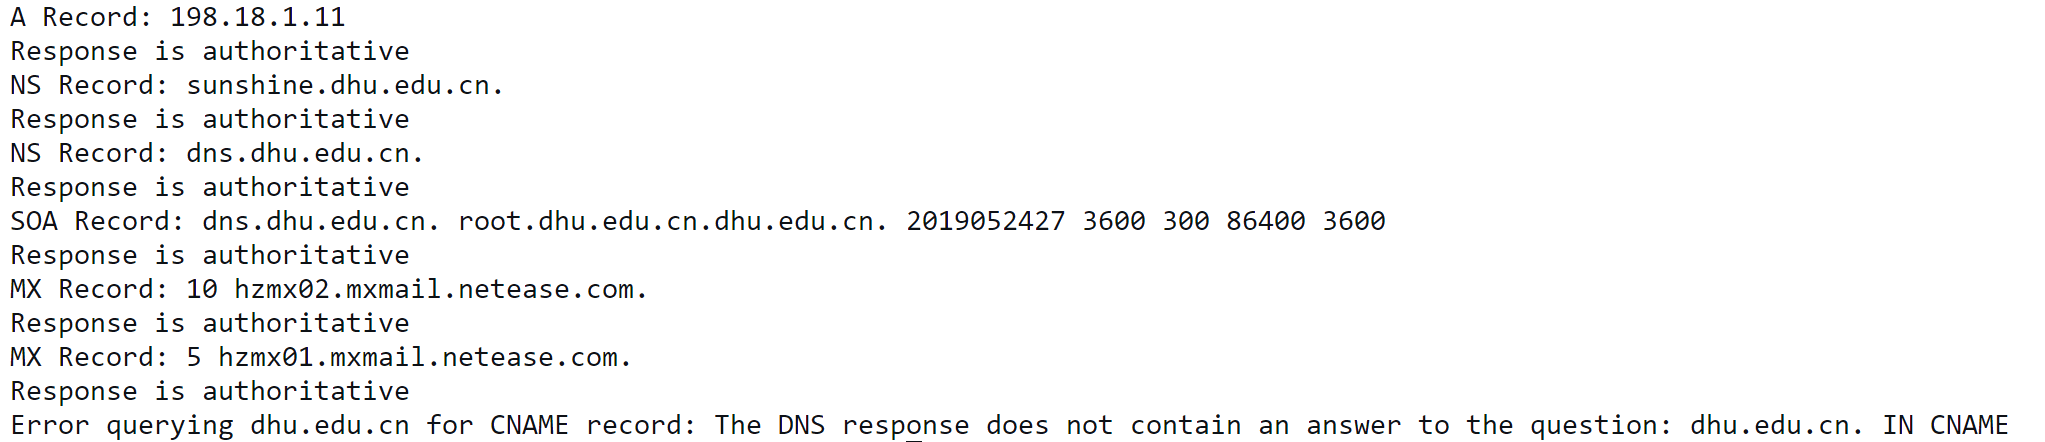
\includegraphics{img/8.2.png}}
 \caption{对dhu.edu.cn的DNS解析结果}
 \label{}
\end{figure}

\clearpage

\section{项目9:网络爬虫}

\subsection{项目描述}
本项目的目标是开发一个网络爬虫,用于从特定网站下载 PDF 文件。网络爬虫是一种自动化工具,可以在互联网上浏览网页并下载数据。在本项目中,我们将重点放在寻找和下载网页上的 PDF 文档。

\subsection{项目实现思路}
项目使用 Python 语言,并利用 requests 库来发送网络请求,以及 BeautifulSoup 库来解析 HTML。程序将访问给定的网址,寻找指向 PDF 文件的链接,并下载这些文件。下载的文件将保存在本地指定的文件夹中。

\subsection{项目代码}
以下是实现网络爬虫的 Python 代码:

\begin{minted}[frame=lines,framesep=2mm,baselinestretch=1.2,fontsize=\footnotesize,linenos]{python}
import requests
from bs4 import BeautifulSoup
import re
import os

def download_pdf(url, folder="downloaded_pdfs"):
    headers = {
        'User-Agent': 'Mozilla/5.0 (Windows NT 10.0; Win64; x64) AppleWebKit/537.36 (KHTML, like Gecko) 
        Chrome/58.0.3029.110 Safari/537.3'
    }

    response = requests.get(url, headers=headers)
    if response.status_code != 200:
        print("Failed to retrieve the page")
        return

    soup = BeautifulSoup(response.text, 'html.parser')
    pdf_links = soup.find_all('a', href=re.compile(r'/(details|download)/[^\s]+\.pdf'))

    if not os.path.exists(folder):
        os.makedirs(folder)

    for link in pdf_links:
        pdf_url = 'https://archive.org' + link.get('href')
        pdf_response = requests.get(pdf_url, headers=headers)
        pdf_name = pdf_url.split('/')[-1]

        with open(f"{folder}/{pdf_name}", 'wb') as file:
            file.write(pdf_response.content)
        print(f"Downloaded {pdf_name}")

download_pdf("https://archive.org/details/networking-books")
\end{minted}

\subsection{实验结果}
实验结果将展示从指定网站成功下载的 PDF 文件的列表。每个下载的文件将在控制台中打印其名称,提供明确的反馈,证明爬虫工作正常。
\begin{figure}[H]
\centering
 \resizebox{0.75\textwidth}{!}{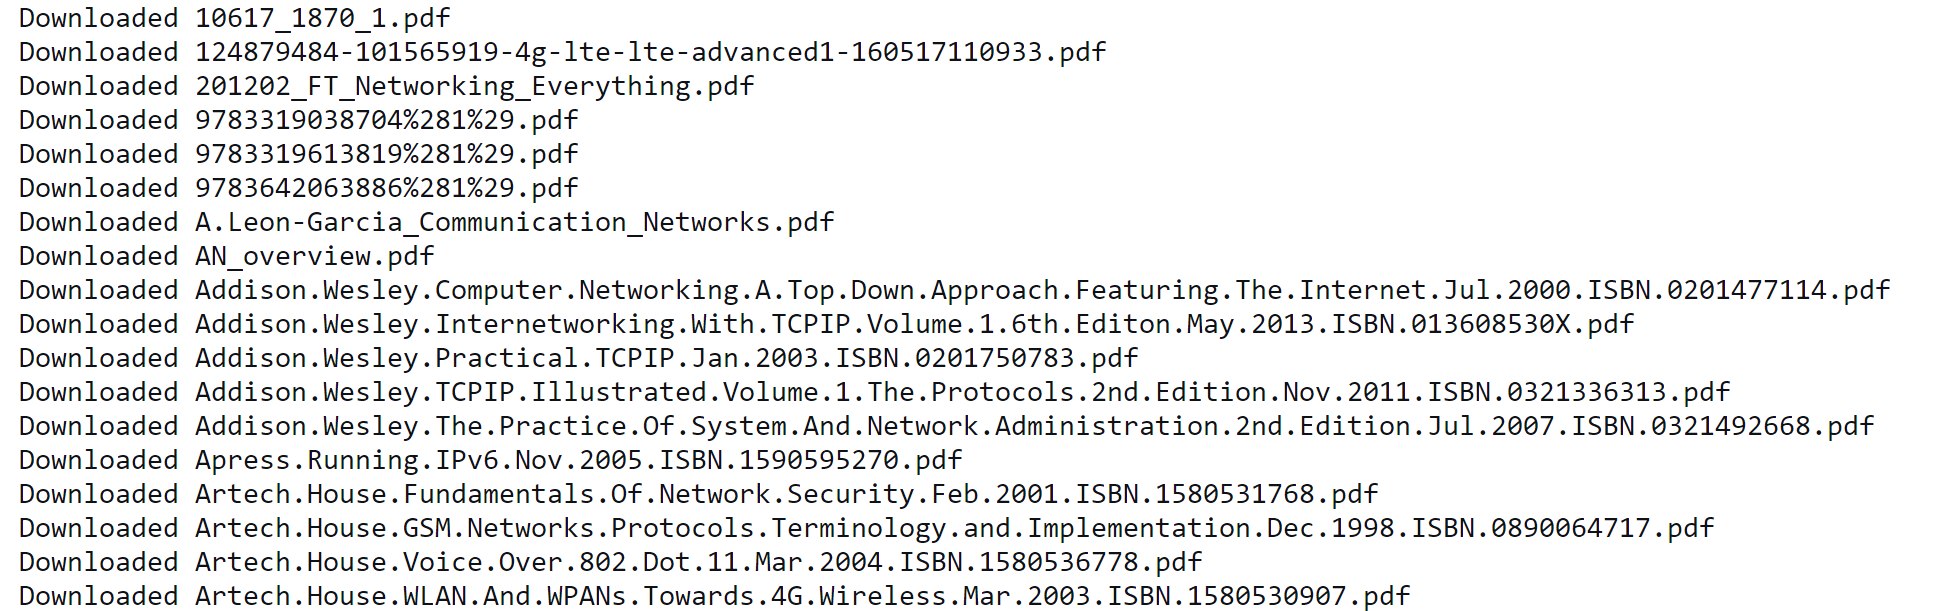
\includegraphics{img/9.1.png}}
 \caption{网络爬虫结果}
 \label{}
\end{figure}

\begin{figure}[H]
\centering
 \resizebox{0.65\textwidth}{!}{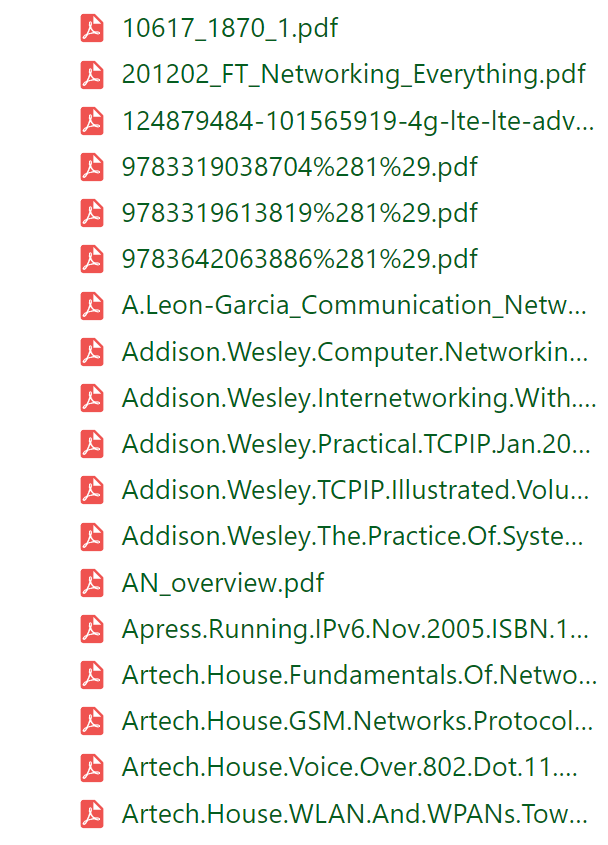
\includegraphics{img/9.2.png}}
 \caption{下载的PDF文件}
 \label{}
\end{figure}
\clearpage
\section{项目10:点对点文件传输系统}
\subsection{项目描述}
本项目的目的是开发一个点对点的文件传输系统,允许用户通过 IPv4 网络进行文件的发送和接收。文件传输是网络编程中的一个基本功能,对于理解网络通信的底层机制非常重要。

\subsection{项目实现思路}
项目分为两部分:文件接收(receive.py)和文件发送(send.py)。接收端使用 Python 的 socket 库在指定端口监听传入的连接,并接收发送端传来的文件。发送端同样使用 socket 库连接到接收端的 IP 地址和端口,并发送文件数据。整个过程使用 TCP 协议确保数据传输的可靠性。

\subsection{项目代码}
以下是实现文件传输的 Python 代码:

\subsubsection{receive.py}
\begin{minted}[frame=lines,framesep=2mm,baselinestretch=1.2,fontsize=\footnotesize,linenos]{python}
import socket
import time

def receive_file_ipv4(port):
    s = socket.socket(socket.AF_INET, socket.SOCK_STREAM)
    s.bind(('0.0.0.0', port))
    s.listen(5)
    print(f"服务器启动,监听端口 {port}...")

    conn, addr = s.accept()
    print(f"来自 {addr} 的连接已建立")

    # 接收文件名
    filename_length_bytes = conn.recv(4)
    filename_length = int.from_bytes(filename_length_bytes, 'big')
    filename_bytes = conn.recv(filename_length)
    filename = filename_bytes.decode('utf-8')
    print(f"接收文件名: {filename}")

    # 接收文件数据
    with open(filename, 'wb') as f:
        print("接收数据中...")
        total_bytes_received = 0
        start_time = time.time()
        while True:
            data = conn.recv(65536)
            if not data:
                break
            bytes_received = len(data)
            total_bytes_received += bytes_received
            f.write(data)

            # 计算每秒的接收速度
            current_time = time.time()
            elapsed_time = current_time - start_time
            if elapsed_time > 0:
                speed = total_bytes_received / elapsed_time / (1024 * 1024)
                print(f"\r当前接收速度: {speed:.2f} Mb/秒", end='', flush=True)

    print("\n文件接收完毕")
    conn.close()
    s.close()

receive_file_ipv4(12345)
\end{minted}

\subsubsection{send.py}
\begin{minted}[frame=lines,framesep=2mm,baselinestretch=1.2,fontsize=\footnotesize,linenos]{python}
import socket

def send_file_ipv4(filename, target_ip, port):
    s = socket.socket(socket.AF_INET, socket.SOCK_STREAM)
    s.connect((target_ip, port))

    # 发送文件名
    filename_bytes = filename.encode('utf-8')
    filename_length = len(filename_bytes)
    s.sendall(filename_length.to_bytes(4, 'big'))  # 发送文件名长度(4字节)
    s.sendall(filename_bytes)  # 发送文件名

    # 发送文件数据
    with open(filename, 'rb') as f:
        print("发送数据中...")
        while True:
            data = f.read(65536)
            if not data:
                break
            s.send(data)

    print("文件发送完毕")
    s.close()

send_file_ipv4('Task07/yolov5s.pt', '10.206.17.20', 12345)
\end{minted}

\subsection{实验结果}
实验结果将展示文件发送和接收的过程,包括文件名的传输、文件数据的传输以及传输速度的计算。这些结果有助于验证文件传输系统的功能和效率。
\begin{figure}[H]
\centering
 \resizebox{0.75\textwidth}{!}{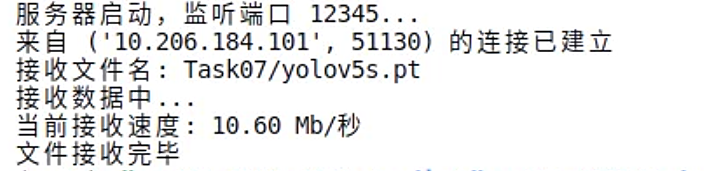
\includegraphics{img/10.1.png}}
 \caption{文件接收端结果}
 \label{}
\end{figure}

\begin{figure}[H]
\centering
 \resizebox{0.35\textwidth}{!}{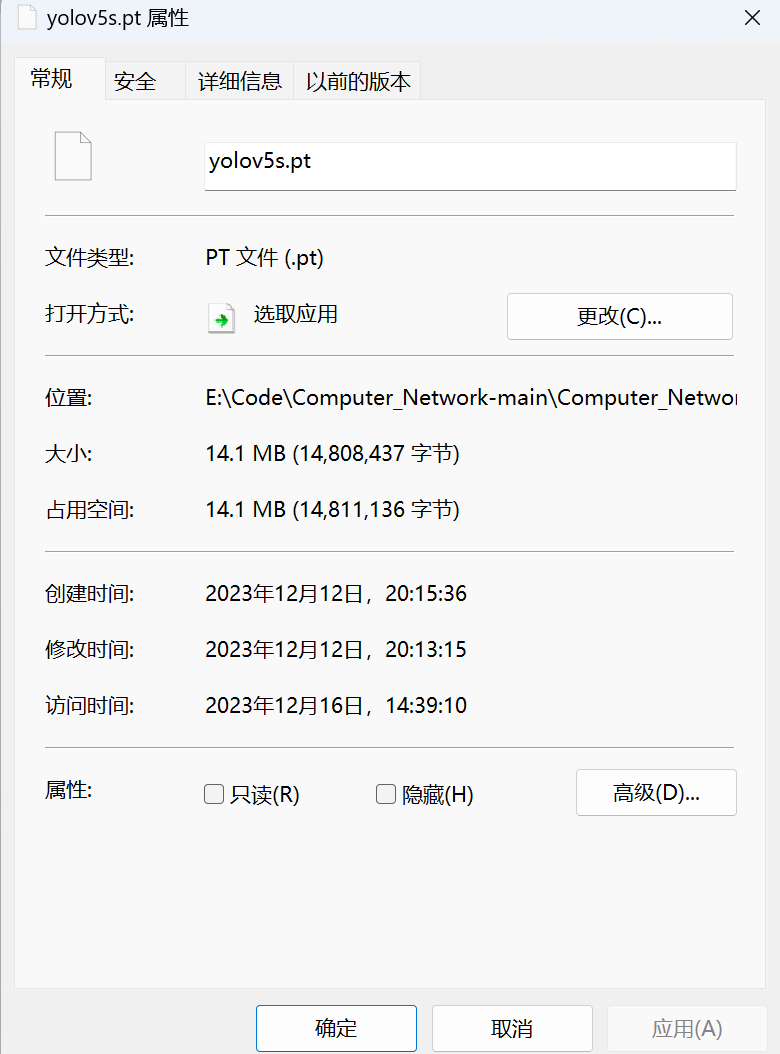
\includegraphics{img/10.2.png}}
 \caption{发送文件信息}
 \label{}
\end{figure}

\begin{figure}[H]
\centering
 \resizebox{0.35\textwidth}{!}{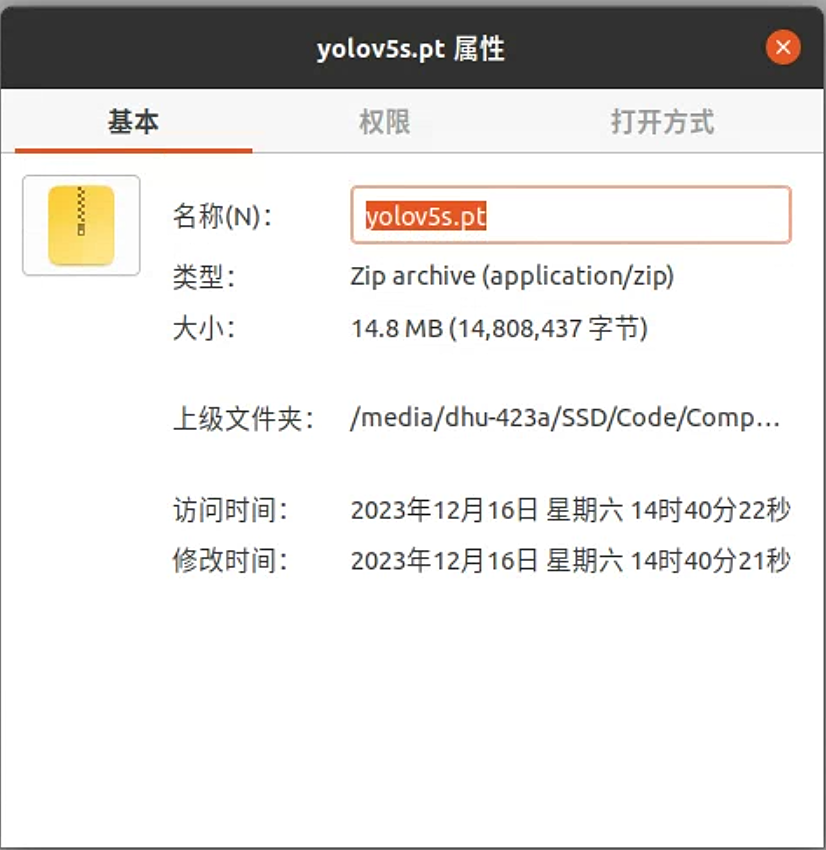
\includegraphics{img/10.3.png}}
 \caption{接受的文件信息}   
 \label{}
\end{figure}

\clearpage

\section{总结}
在这系列的项目中,我深入探索了多种计算机网络和编程领域的关键概念和技术。每个项目都是针对特定的技术挑战设计的,从基础的子网划分和 TCP/IP 协议的具体实现,到更高级的网络服务如 DNS 解析和文件传输。通过这些项目,我不仅加深了对理论知识的理解,还获得了实际应用这些知识的经验

\end{document}